\begin{center}
\Huge
Punkter og vektorer
\end{center}

\section*{Vektorer mellem punkter}
\stepcounter{section}
Har vi to punkter $A(a_1,a_2)$ og $B(b_1,b_2)$, så betegner vi vektoren mellem punkterne som
\begin{align*}
\vv{AB}.
\end{align*}
Vi kalder denne vektor for \textit{forbindelsesvektoren} fra $A$ til $B$.
Vi definerer derfor koordinaterne til vektoren $\vv{AB}$ ved 
\begin{align*}
	\vv{AB} = 
	\begin{pmatrix}
		b_1 - a_1\\b_2-a_2
	\end{pmatrix}.
\end{align*}
Som et vigtigt eksempel har vi vektoren fra punktet origo $O(0,0)$ til et punkt $P(p_1,p_2)$, der betegnes 
\begin{align*}
\vv{OP},
\end{align*}
og kaldes for \textit{stedvektoren} for $P$. 
Koordinaterne til vektoren $\vv{OP}$ er givet ved 
\begin{align*}
	\vv{OP} = 
	\begin{pmatrix}
		p_1\\p_2
	\end{pmatrix}.
\end{align*}
\begin{exa}
Stedvektoren til punktet $P(2,3)$ er givet ved 
\begin{align*}
	\vv{OP} = 
	\begin{pmatrix}
		2\\3
	\end{pmatrix}.
\end{align*}
Har vi også punktet $Q(-3,5)$, så er vektoren $\vv{PQ}$ givet ved
\begin{align*}
	\vv{PQ} =
	\begin{pmatrix}
		-3-2\\
		5-3
	\end{pmatrix} =
	\begin{pmatrix}
		-5\\2
	\end{pmatrix}.
\end{align*}
\end{exa}

\section*{Længde af vektor}

Vi ønsker at definere længden af en vektor. 
\begin{defn}[Længden af en vektor]
	Længden af en vektor $\vv{v}$ med koordinaterne
	\begin{align*}
		\vv{v} = 
		\begin{pmatrix}
			v_1 \\ v_2
		\end{pmatrix}
	\end{align*}
	defineres som
	\begin{align*}
		|\vv{v}| = \sqrt{v_1^2 + v_2^2}.
	\end{align*}
\end{defn}
Den opmærksomme læser vil nok bemærke længdeformlens lighed med Pythagoras' sætning. 

\begin{exa}
	Vektoren $\vv{v}$ givet ved
	\begin{align*}
		\vv{v} = 
		\begin{pmatrix}
			-6 \\ 8
		\end{pmatrix}
	\end{align*}
	har længden 
	\begin{align*}
		|\vv{v}| = \sqrt{(-6)^2+8^2} = \sqrt{36+64} = \sqrt{100} = 10
	\end{align*}
\end{exa}

\begin{setn}[Afstand mellem to punkter]
Skal vi bestemme afstanden mellem et punkt $P = (p_1,p_2)$ og et punkt $Q = (q_1,q_2)$, så er det givet ved
\begin{align*}
\texttt{dist}(P,Q) = |\vv{PQ}| = \sqrt{(p_1-q_1)^2+(p_2-q_2)^2}
\end{align*}
\end{setn}
\begin{proof}
Vektoren $\vv{PQ}$ er givet ved
\begin{align*}
\vv{PQ}=\begin{pmatrix}
q_1-p_1\\q_2-p_2
\end{pmatrix}.
\end{align*}
Vi anvender nu blot formlen for længden af en vektor og får
\begin{align*}
|\vv{PQ}| = \sqrt{(q_1-p_1)^2+(q_2-p_2)^2}
\end{align*}
\end{proof}
\begin{exa}
Afstanden fra punktet $P(0,1)$ og punktet $Q(-1,2)$ er givet ved
\begin{align*}
\texttt{dist}(P,Q) = \sqrt{(-1-1)^2+(2-1)^2} = \sqrt{5}.
\end{align*}
\end{exa}


\subsection*{Opgave 1}
	\begin{figure}[H]
		\centering
		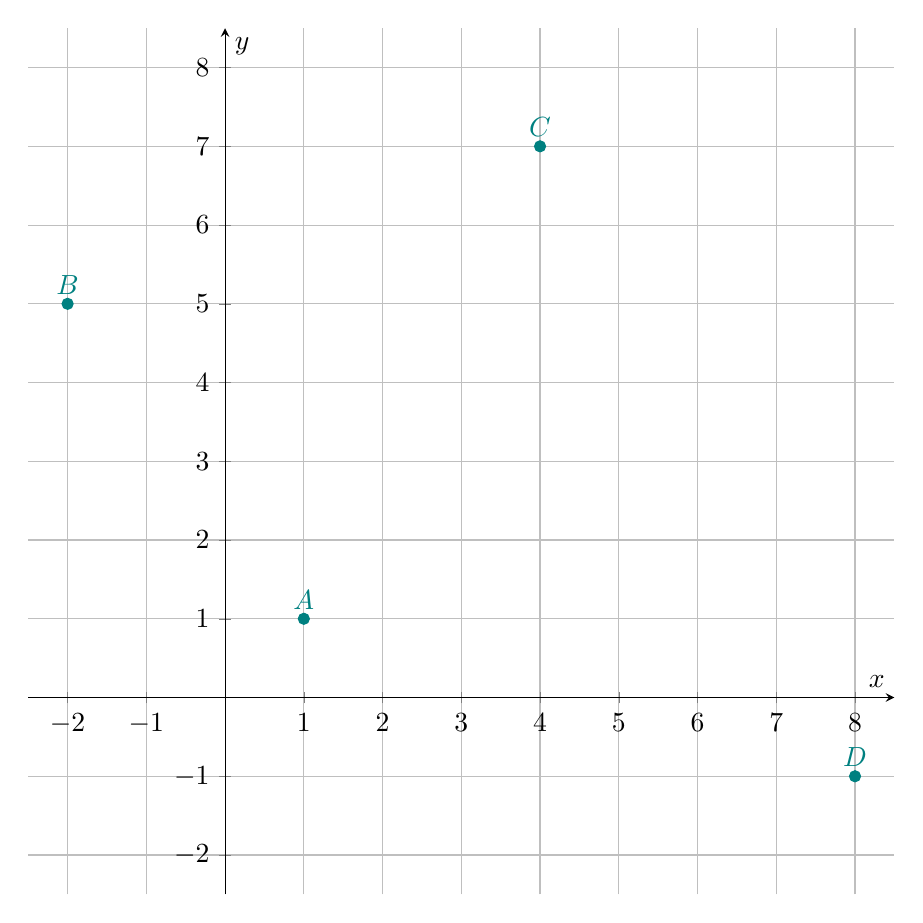
\begin{tikzpicture}
			\begin{axis}[
				axis lines = middle, 
				xmin = -2.5, xmax = 8.5,
				ymin = -2.5, ymax = 8.5,
				x = 1cm, y = 1cm,
				grid,
				xlabel = $x$, ylabel = $y$
			]
			\filldraw[teal] (axis cs: 1,1) circle (2pt) node[above] {$A$};
			\filldraw[teal] (axis cs: -2,5) circle (2pt) node[above] {$B$};
			\filldraw[teal] (axis cs: 4,7) circle (2pt) node[above] {$C$};
			\filldraw[teal] (axis cs: 8,-1) circle (2pt) node[above] {$D$};
			\end{axis}
		\end{tikzpicture}
		\caption{Repræsentanter for to vektorer}
		\label{fig:tovektorer}
	\end{figure}
\begin{enumerate}[label = \roman*)]
	\item Bestem koordinaterne for punkterne $A$, $B$ $C$ og $D$.
	\item Bestem koordinaterne til vektorerne $\vv{AB}$, $\vv{BC}$, $\vv{DA}$ og $\vv{BD}$.
	\item Bestem længden af vektorerne $\vv{AB}$, $\vv{BC}$, $\vv{DA}$ og $\vv{BD}$.
\end{enumerate}

\subsection*{Opgave 2}
\begin{enumerate}[label = \roman*)]
	\item For punkterne $A(2,5)$ og $B(4,9)$ kan du så uden at tegne punkterne gennemskue hvad
	koordinaterne til forbindelsesvektoren $\vv{AB}$ bliver?
	\item Hvis vi har to punkter $A(a_1,a_2)$ og $B(b_1,b_2)$, kan du så gennemskue, hvordan vi
	udregner koordinaterne til forbindelsesvektoren $\vv{AB}$?
\end{enumerate}


\subsection*{Opgave 3}

Bestem koordinaterne til stedvektoren til følgende punkter 
\begin{align*}
&1) \ (1,2)   &&2) \  (3,-1)  \\
&3) \  (\sqrt{2},\sqrt{5})  &&4) \ (-2,7)    \\
\end{align*}


\subsection*{Opgave 4}
Fire punkter er givet ved $A(1,3)$, $B(-5,6)$, $C(-4,1)$ og $D(12,-7)$.
\begin{enumerate}[label = \roman*)]
	\item Bestem koordinaterne til vektorerne $\vv{AB}$, $\vv{BC}$ og $\vv{DA}$.
	\item Bestem længden af vektorerne $\vv{AB}$, $\vv{BC}$ og $\vv{DA}$
	\item Bestem $\vv{BA} + \vv{CD}$.
	\item Bestem $|2\vv{CA} - 3\vv{BC} + \vv{DB}|$.
\end{enumerate}

\subsection*{Opgave 5}
Bestem afstanden mellem punkterne $A(6,3)$ og $B(9,7)$.
